\documentclass[12pt]{article}
\usepackage{amsmath}
\usepackage[export]{adjustbox}
\usepackage{unicode}
\usepackage[table]{xcolor}
\usepackage{longtable}
\usepackage{pdflscape}
\usepackage{siunitx}
\usepackage{setspace}
\usepackage[scaled]{helvet}
\renewcommand\familydefault{\sfdefault} 
\usepackage[T1]{fontenc}
\usepackage[numbers]{natbib} 
\usepackage{tabularx}
\usepackage[hidelinks]{hyperref} 
\hypersetup{ colorlinks, citecolor=black,
  filecolor=black, 
  linkcolor=black,
  urlcolor=blue,
  pdftitle={Hardware Design and System Updates},
  pdfpagemode=FullScreen,
}
\usepackage{float}
\usepackage{graphicx} 
\usepackage{pdfpages} 
\usepackage{tabularx}
\usepackage{tikz}
\newcommand\createfigurew[3]{
  \begin{center}
  \begin{figure}[H]
    \centering \includegraphics[width=\textwidth]{#1}
    \caption{#2}
    \label{#3}
  \end{figure}
  \end{center}
}
\newcommand\createfigurel[3]{
  \begin{center}
  \begin{figure}[H]
    \centering \includegraphics[height=0.8\textheight]{#1}
    \caption{#2}
    \label{#3}
  \end{figure}
  \end{center}
}
\usepackage{etoolbox}
\apptocmd{\thebibliography}{\raggedright}{}{}
\begin{document}
\linespread{1.0}
\begin{titlepage}
  \begin{center}
    \large{University of Puerto Rico\\
    Mayagüez Campus\\
    \vspace{\baselineskip}
    Department of Electrical and Computer Engineering\\}
    \vspace{6cm}
    \Huge{\underline{Insulin Temperature Warning System}\\}
    \vspace{0.5\baselineskip}
    \large by\\
    Fabio J. Matos Nieves\\
    Enrique Chompré\\
    Guillermo Colón\\
    Rubén Marrero\\
    \vspace{3.5cm}
    For: Professor Manuel Jimenez\\
    Course: INEL 4217 Seccion 096\\
    Date: Febuary 2, 2023\\
    \normalsize

  \end{center}
\end{titlepage}

\linespread{2.0}
\tableofcontents
\listoffigures
\listoftables
\section{Delegation of Tasks}
For this proposal, the Insulin Temperature Warning System was modulerized into 3 separate parts, those being:
\begin{itemize}
  \item Main Unit
  \item Sub Unit
  \item PSU
\end{itemize}
The main unit consists of the MSP430FR2110 and the HM-10 BLE Bluetooth module. The sub unit consists of MSP430FR2000, a HM-10 BLE Bluetooth module and a red LED. The PSU consists of 2 individual parts:
\begin{itemize}
  \item Main Unit PSU
  \item Sub unit PSU
\end{itemize}
The main unit consists of a 3.3\si{\V} power supply along with a 3.3\si{\V} voltage sense for a GPIO pin with a battery backup circuit.  The sub unit PSU consists of a 3.3\si{\V} regulated battery supply.\\
The following table demonstrates how the modules were distributed within the team:
\begin{table}[h]
\begin{center}
\begin{tabularx}{\textwidth}{|X|X|}
 \hline
 Team Member & Assigned Module\\
 \hline
 Fabio J. Matos Nieves & PSU\\
 \hline
 Enrique Chompré González& Main Unit\\
 \hline
 Guillermo Colón Bernardi& Sub Unit\\
 \hline
\end{tabularx}
\end{center}
\caption{Team Member Roles}
\label{Task-Delegation}
\end{table}

\section{Updated Block Diagram}
\createfigurewsvg{../BDv3/Figures/bdv3-main.svg}{Main Unit Architectural Diagram}{fig:main-bdv3}
\createfigurewsvg{../BDv3/Figures/bdv3-sub.svg}{Sub Unit Architectural Diagram}{fig:sub-bdv3}

\section{System Schematic Diagrams}
\begin{landscape}
  \begin{center}
  \begin{figure}[H]
    \centering 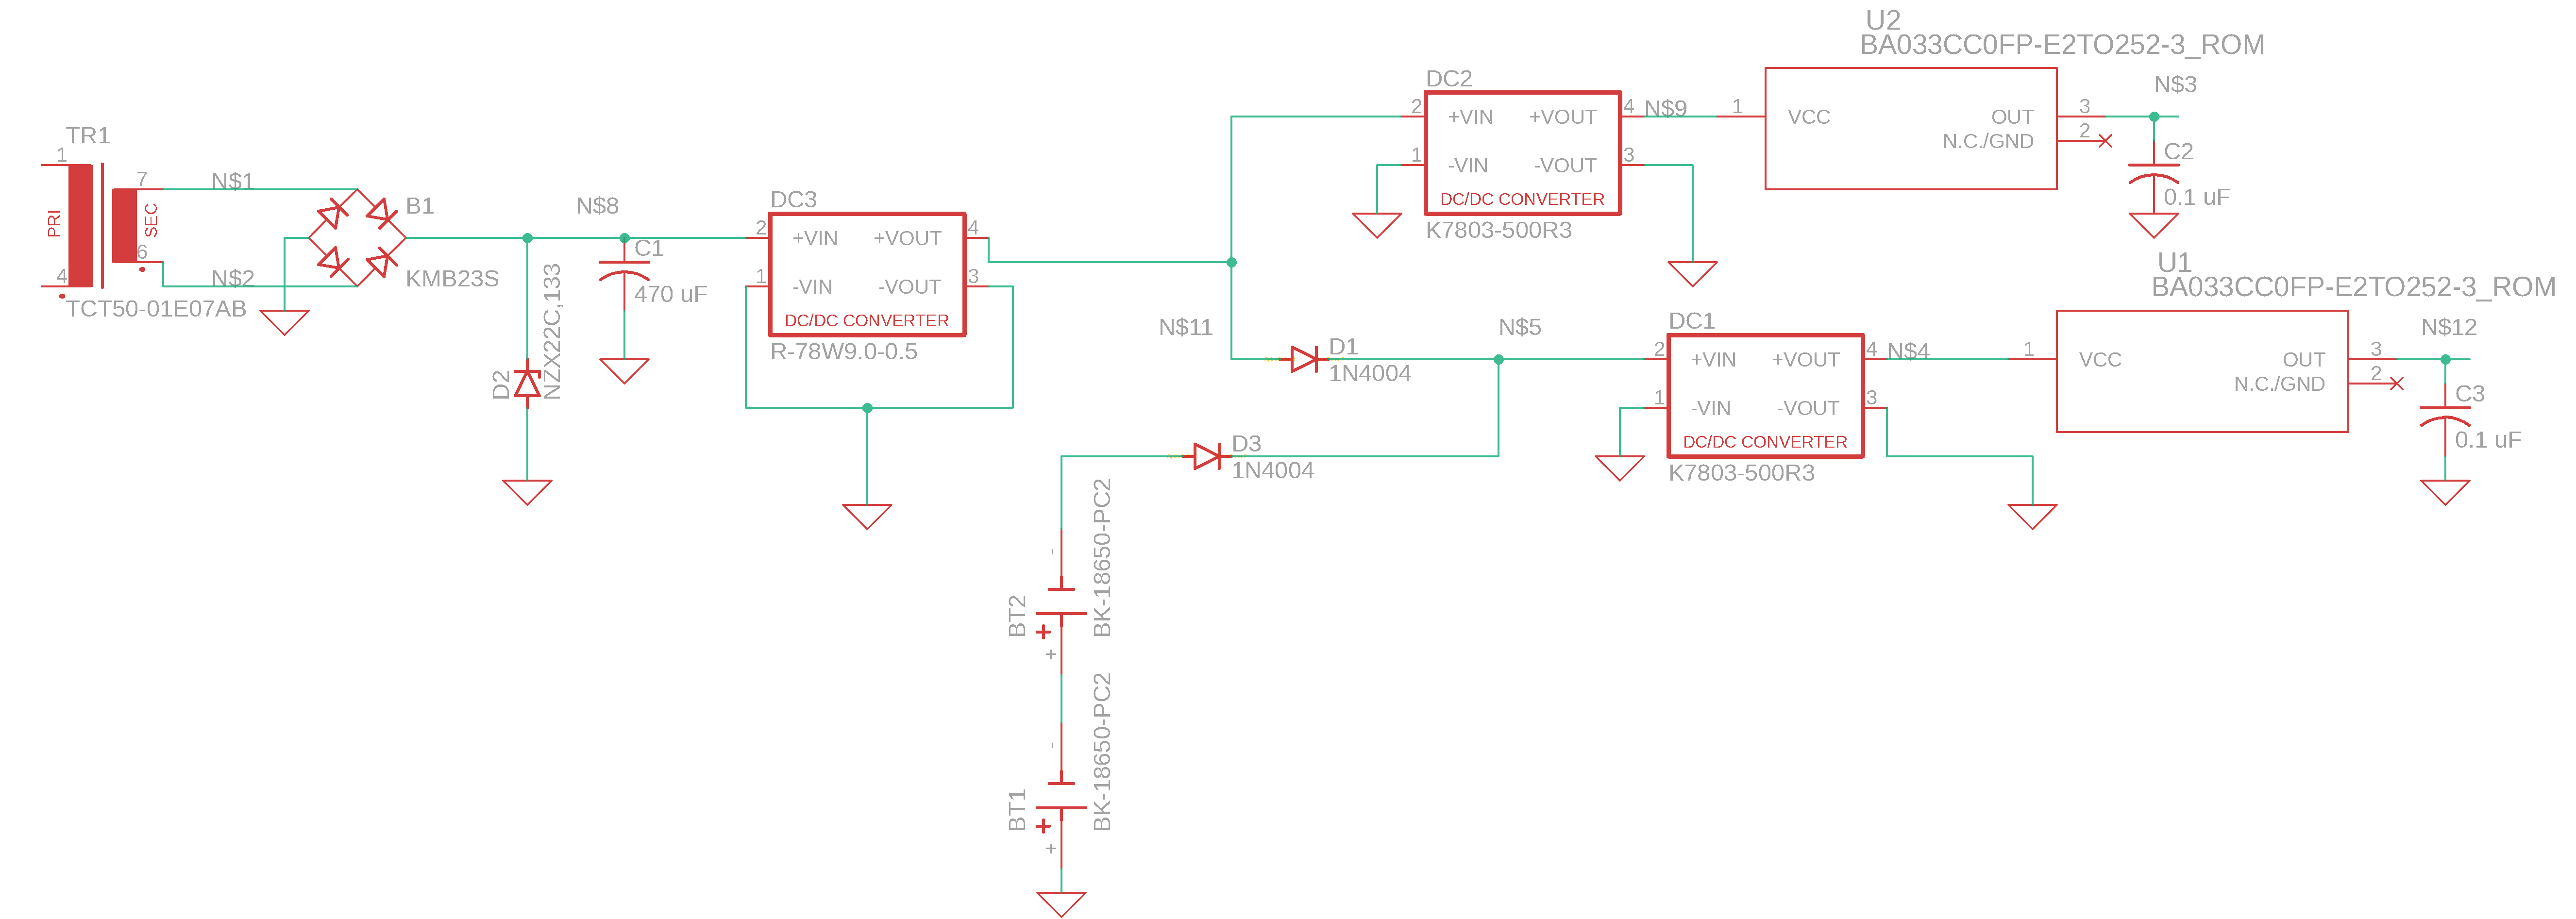
\includegraphics[width=1.6\textwidth]{../Power-Supply/Main Unit PSU/main-unit-psu.png}
    \caption{Main Unit PSU Schematic}
    \label{fig:main-psu-schematic}
  \end{figure}
  \end{center}
\end{landscape}
\createfigurew{../Power-Supply/Sub Unit PSU/sub-unit-psu.png}{Sub Unit PSU Schematic}{fig:sub-psu-schematic}
\createfigurew{../Main-Unit/Figures/Main-Unit.png}{Main Unit Schematic}{fig:main-unit-schematic}
\createfigurew{../Sub-Unit/Figures/sub-unit.png}{Sub Unit Schematic}{fig:Sub-unit-schematic}
\begin{landscape}
  \begin{center}
  \begin{figure}[H]
    \centering 
\includegraphics[width=1.5\textwidth]{../Main-Unit-and-PSU/Figures/main-unit-and-psu.png}
    \caption{Main Unit with PSU Schematic}
    \label{fig:main-with-psu-schematic}
  \end{figure}
  \end{center}
\end{landscape}

\begin{landscape}
\section{Bill of Materials}
\begin{center}
  \begin{table}[h]
    \addtocounter{table}{-1}
  \begin{longtable}[c]{|c|c|c|c|c|c|c|c|c|}
    \hline
    \multicolumn{9}{|c|}{Bill of Materials: Main Unit}\\
    \hline
    Item\#&Qty&Description&Ref&Part\#&Unit Price&Est. Cost&Supplier&Datasheet\\
    \hline
    1&1&120-24 \si{\V} Transformer&TR1&TCT50-01E07AB&\$10.02&\$10.02&\href{https://www.digikey.com/en/products/detail/triad-magnetics/TCT50-01E07AB/2688350}{Digi-Key}&\href{http://catalog.triadmagnetics.com/Asset/TCT50-01E07AB.pdf}{Data-sheet}\\
    \hline
    2&1&Diode Rectifier&B1&KMB23S&\$0.47&\$0.47&\href{https://www.digikey.com/en/products/detail/smc-diode-solutions/KMB23S/7898339}{Digi-Key}&\href{https://www.smc-diodes.com/propdf/KMB22S\%20THRU\%20KMB220S\%20N1952\%20REV.B.pdf}{Data-sheet}\\
    \hline
    3&1&9 \si{\V} Zener Diode&D2&NZX9V1B,133&\$0.20&\$0.20&\href{https://www.digikey.com/en/products/detail/nexperia-usa-inc/NZX9V1B-133/2119779}{Digi-Key}&\href{https://assets.nexperia.com/documents/data-sheet/NZX_SER.pdf}{Data-sheet}\\
    \hline
    4&1&10\si{\micro\farad} 25\si{\V} Capacitor&C1&ESW106M025AC3AA&\$0.27&\$0.27&\href{https://www.digikey.com/en/products/detail/kemet/ESW106M025AC3AA/13176208?s=N4IgTCBcDaIBwHYCCBhOBGArJkBdAvkA}{Digi-Key}&\href{https://api.kemet.com/component-edge/download/datasheet/ESW106M025AC3AA.pdf}{Data-sheet}\\
    \hline
    5&1&9\si{\V} DC-DC Converter&DC3&R-78W5.0-0.5&\$10.37&\$10.37&\href{https://www.digikey.com/en/products/detail/recom-power/R-78W9-0-0-5/4930587?s=N4IgTCBcDaIEoFoDsAOA6gTgHQAYE6wFYQBdAXyA}{Digi-Key}&\href{https://recom-power.com/pdf/Innoline/R-78W-0.5.pdf}{Data-sheet}\\
    \hline
    6&2&Regular Diode&D1,D3&1N4004&\$0.10&\$0.20&\href{https://www.digikey.com/en/products/detail/nte-electronics-inc/1N4004/11645015}{Digi-Key}&\href{https://www.digikey.com/en/products/detail/nte-electronics-inc/1N4004/11645015}{Data-sheet}\\
    \hline
    7&2&3.7 Battery&BT1,BT2&ICR18650-2200-F&\$5.00&\$5.00&\href{https://www.digikey.com/en/products/detail/pkcell/ICR18650-2200-F/11629982?s=N4IgTCBcDaIJIGEBKBGAHANgKwAYC0YYO\%2BAYiALoC\%2BQA}{Digi-Key}&\href{https://media.digikey.com/pdf/Data\%20Sheets/FusPower\%20PDF's/ICR18650_2200.pdf}{Data-sheet}\\
    \hline
    8&2&3.3\si{\V} DC-DC Converter&DC1,DC2&K7803-500R3&\$2.26&\$4.52&\href{https://www.digikey.com/en/products/detail/mornsun-america-llc/K7803-500R3/13168320}{Digi-Key}&\href{https://www.mornsun-power.com/html/pdf/K7803-500R3.html}{Data-sheet}\\
    \hline
    9&2&3.3\si{\V} LDO&U1-U2&BA033CC0FP-E2&\$1.41&\$2.42&\href{https://www.digikey.com/en/products/detail/rohm-semiconductor/BA033CC0FP-E2/722186?s=N4IgTCBcDaIEIEEAMBmFBhdSBiAFAtAKIQC6AvkA}{Digi-Key}&\href{https://www.rohm.com/datasheet?p=BA033CC0FP&dist=Digi-key&media=referral&source=digi-key.com&campaign=Digi-key}{Data-sheet}\\
    \hline
  \end{longtable}
  \caption{Bill of Materials: Main Unit}
  \label{BOM:Main-Unit}
  \end{table}
  \begin{table}[h]
    \addtocounter{table}{-1}
  \begin{longtable}[c]{|c|c|c|c|c|c|c|c|c|}
    \hline
    \multicolumn{9}{|c|}{Bill of Materials: Sub Unit}\\
    \hline
    Item\#&Qty&Description&Ref&Part\#&Unit Price&Est. Cost&Supplier&Datasheet\\
    \hline
    1&2&3.7 Battery&BT1,BT2&ICR18650-2200-F&\$5.00&\$10.00&\href{https://www.digikey.com/en/products/detail/pkcell/ICR18650-2200-F/11629982?s=N4IgTCBcDaIJIGEBKBGAHANgKwAYC0YYO\%2BAYiALoC\%2BQA}{Digi-Key}&\href{https://media.digikey.com/pdf/Data\%20Sheets/FusPower\%20PDF's/ICR18650_2200.pdf}{Data-sheet}\\
    \hline
    2&1&3.3\si{\V} DC-DC Converter&DC1&K7803-500R3&\$2.26&\$2.26&\href{https://www.digikey.com/en/products/detail/mornsun-america-llc/K7803-500R3/13168320}{Digi-Key}&\href{https://www.mornsun-power.com/html/pdf/K7803-500R3.html}{Data-sheet}\\
    \hline
    3&1&3.3\si{\V} LDO&U1&BA033CC0FP-E2&\$1.41&\$1.41&\href{https://www.digikey.com/en/products/detail/rohm-semiconductor/BA033CC0FP-E2/722186?s=N4IgTCBcDaIEIEEAMBmFBhdSBiAFAtAKIQC6AvkA}{Digi-Key}&\href{https://www.rohm.com/datasheet?p=BA033CC0FP&dist=Digi-key&media=referral&source=digi-key.com&campaign=Digi-key}{Data-sheet}\\
    \hline
  \end{longtable}
  \caption{Bill of Materials: Sub Unit}
  \label{BOM:Sub-Unit}
  \end{table}
\end{center}
\end{landscape}

\section{Power, voltage compatibility,\\ and Timing Analyses}
\subsection{Main Unit PSU}
According to the TCT50-01E07AB data-sheet \cite{TCT5001E07AB}, given an input voltage of 120$\si{\V}_{RMS}$ AC voltage, it will output a 10$\si{\V}_{RMS}$ AC voltage, thus $N\$1$ and $N\$2$ will have a voltage of -10\si{\V} to 10\si{\V}, depending on which part of the sine wave is currently being supplied. The voltage at the output of the bridge rectifier B1 at $N\$8$ was calculated as follows:
\begin{equation}
  B1_{Out} = N\$1 - V_{BD}
  \label{eq:main-b1out}
\end{equation}
In this design B1 has a drop of 0.55 per element and since there are 2 elements per cycle this means $V_{BD}$ is equal to 1.1\si{V} \cite{KMB23S}. This means that equation \ref{eq:main-b1out} is 22.9\si{\V} for this design. Then the voltage at $N\$8$ is rectified to 22.8\si{V} by D2 (a 22.8\si{\V} zener diode) and is denoised by C1 (a 50\si{\V} 470\si{\micro\farad} capacitor) which was calculated as follows:
\begin{equation}
  V_{PP} = \frac{I}{2fC}
  \label{eq:main-filter-cap}
\end{equation}
$V_{PP}$ is the peak-to-peak ripple voltage, $I$ is the current in the circuit, $f$ is the source frequency of the AC power and $C$ is the capacitance of the selected capacitor. Given that equation \ref{eq:main-b1out} is equal to 22.8 in this design, a ripple voltage of less than 1\% was chosen. To simplify the equations, the in operation current for the Bluetooth module was chosen to represent $I$ which according to the HM-10 data sheet is 8.5\si{\mA} and the rest of the current consuming devices were assumed to be negligible. Given that $f$ is the mains frequency in Puerto Rico and the United States of America, $f$ is 60\si{\Hz}. Solving for C given $\%V_{PP}$ gives the following equation:
\begin{equation}
  C = \frac{I}{2f\%V_{PP}}100
  \label{eq:cap-given-percent-vpp}
\end{equation}
For this design, this equation solves to 310\si{\micro\farad}, which assuming $I$ is accurate a 330\si{\micro\farad} capacitor would suffice but since it was assumed that other current drawing sources besides the Bluetooth module were negligible, this means that $I$ is an underestimate of the true current through the system. Thus a 470\si{\micro\farad} was chosen to account for the underestimation in current.\\\\
$N\$8$ is then fed to $+VIN$ which is compatible with the input voltage since $+VIN_{Min} < N\$8 < +VIN_{Max}$ which are 11\si{\V} and 32\si{\V} respectively \cite{R78W900}.
$N\$11$ was calculated as follows:
\begin{equation}
  N\$11 = DC3_{+VOUT}
  \label{eq:main-N11}
\end{equation}
In this case since $+VOUT$ is the output of a 9\si{\V} DC-DC converter, thus $N\$11$ is at 9\si{V} DC. Since $N\$11$ is at 9\si{V}, $DC2_{+VIN}$ is compatible since $+VIN_{Min} < N\$11 < +VIN_{Max}$ which are 4.75\si{\V} and 36\si{\V} respectively. $N\$9$ is the output of DC2 (a 3.3\si{\V} regulator) and thus will be at 3.3\si{\V} which U2 is compatible since $N\$9$ is less than $VIN_{Max}$ for the BA033CC0FP-E2 of 2.5\si{\V} \cite{BA033CC0FPE2}. Then $N\$3$ will be at 3.3\si{\V} denoised and will serve as the GPIO input mains power sense pin for the MCU.
Going back down to $N\$5$, when mains power is available the voltage at this node is calculated as follows:
\begin{equation}
  N\$5_{Mains} = N\$11 - V_{D}
  \label{eq:main-N5-mains}
\end{equation}
To understand why equation \ref{eq:main-N5-mains} is calculated this way, we need first see how BT1, BT2 and D3 interact with each other. BT1 and BT2 are both 3.7\si{\V} 18650 cells \cite{ICR186502200F} in series, thus the voltage at the input of D3 will 7.4\si{\V}. The diode drop for D3 is 1.0\si{\V} \cite{1N4004}, this means that the potential difference at $N\$6$ by the batteries is 6.4\si{\V}. The potential difference by $N\$11$ is 8\si{\V}, thus the voltage difference between the output of DC3 minus $V_{D}$ of D1 and the voltage of the batteries minus $V_{D}$ is 1.6\si{\V}. This means that the D3 will be placed in reverse bias and therefor the batteries will not conduct. When mains power is available, $DC1_{+VINMin} < N\$5 < DC1_{+VINMax}$, this making it compatible with DC1 \cite{K7803500R3}. Since $N\$4$ is the same as $N\$9$, U1 is compatible. The output of U1 ($N\$12$) will serve as the VCC for the MCU.
When mains power is not available, initially $N\$5$ but instantaneously D3 is placed in forward bias and the batteries can conduct, and as calculated above $N\$5$ will be at 6.4\si{\V} which is sufficient to power DC1 and U1.\\\\
At $N\$3$ and $N\$12$ a 0.1\si{\micro\farad} 50\si{\V} capacitor were placed in parallel with the load as a bypass capacitor in order to ensure a clean DC source at both VCC and power sense pin of the MCU. The value of 0.1\si{\micro\farad} was chosen since it is a common value for bypass capacitors for microcontrollers.
\subsection{Sub Unit PSU}
$N\$6$ will be at $2V_{BATT}$, this is due to BT1 and BT2 being in series and each cell is 3.7\si{\V} \cite{ICR186502200F} and thus $N\$6$ will be at 7.4\si{\V}. Since $N\$6$ is at 7.4\si{\V}, it is in the compatible voltage range for DC1 \cite{BA033CC0FPE2}. At $N\$4$ the voltage will be regulated by DC1 and thus will be at 3.3\si{\V}, not exceeding the maximum voltage rating for U1 \cite{BA033CC0FPE2}. $N\$1$ will serve as the regulated output for the MCU.
\subsection{Main Unit}
The Main Unit consists of the MSP430FR2110IPW16 MCU and the HM-10S-A Bluetooth module. For the MCU, it has an input voltge range from 1.8\si{\V} to 3.6\si{\V} according to it's datasheet \cite{Citation}. Meanwhile, the HM-10S-A Bluetooth module has an input voltage from 2.5\si{\V} to 3.3\si{\V} according to it's datasheet \cite{Citation}. Due to this, both devices can handle the input voltage of 3.3\si{\V}, which will be the most optimal voltage for the MSP430FR2110, and will be the maximum voltage the HM-10S-A can handle without having problems while in operation. In order to connect both devices to each other, for comunication, the best protocol to use will be UART. The MSP430FR2110 has 4 pins for UART communication using the eUSCI modules, which can detect automatically the baud-rate to be used. According to the datasheet for the HM-10S-A module\cite{Citation}, it can select the baud-rate to be used, which ranges from a minimum 1200 to a maximum of 230400. In the datasheet of the MSP430FR2110, the eUSCI clock frequency, UART mode, can reach a maximum of 5MHz, which means it can reach the maximum baud-rate of the bluetooth module and can also select lower baud-rates, according to the formula:
\begin{equation}
	Clk Frequency= Baud-rate * 16
	\label{eq:UART Frequency}
\end{equation}
This means if we select the maximum baud-rate of the HM-10S-A module, which is 230400, using the formula, we would need a a frequency of 3.68MHz, which is still below the maximum frequency the eUSCI module on the MSP430FR2110. This will allow us to be able to use the HM-10S-A communicate via UART with the MSP430FR2110. 
\subsection{Sub Unit Voltage \& Baud Rate}
In order to validate the compatibility of MCU MSP430FR2000IPW16 and Bluetooth module HM-10S with respect to their voltage levels and communication protocols, it is necessary to verify their respective related specifications.\\\\
The MSP430FR2000IPW16 component showcases flexibility in terms of voltage adaptability, functioning within a supply range stretching from 1.8V to 3.6V as seen in page 1 from it’s datasheet [CITE HERE]; on the other hand, the HM-10S Bluetooth module has a good operational capacity that ranges from 2.5Volts all the way up to 3.3Volts as shown in page 1 of the HM-10S datasheet [CITE HERE]. Knowing this, it will be needed to power this module via a 3.3V power source so as to satisfy both the voltage requirements for operation alongside those required by MSP430FR2000IPW16 device compatibility guidelines.\\\\
The MSP430FR2000IPW16 is designed to be compatible with various baud rates for serial communication via its Universal Asynchronous Receiver / Transmitter (UART) interface. With a capability of generating 9600 up to 115200 bits per second (bps), it can facilitate efficient data transmission. The HM-10S Bluetooth module also uses UART, and the supported range of baud rates from the datasheet of the HM-10S Bluetooth module is within the capabilities of the MSP430FR2000IPW16 micro-controller, hence compatibility exists between them at this level.\\\\
Another aspect that needed the voltage analysis between the MSP430FR2000IPW16 MCU and the SSL-LX3052ID Red LED. Here the voltage requirements for both devices are considered by taking into account their respective voltage needs.\\\\
As previously said, the MSP430FR2000IPW16 operates at a supply voltage range of 1.8V to 3.6V. The voltage requirement of the SSL-LX3052ID Red Led has a forward Voltage of 2.1 V and a maximum continuous forward current of 30mA. Therefore, it needs to be ensured that the LED is powered with a voltage that meets its forward voltage requirement and a current that does not exceed its maximum forward current rating. \\\\
To meet these requirements, it was considered how the LED is connected to the MCU. To control the forward Voltage intensity and the current flowing through the LED, a resistor will be needed between both. To know the R needed for this resistor, the following formula was used:\\\\
\begin{equation}
R = \frac{V_{cc} - V_{f}}{I_{f}}
\end{equation}
Where Vcc is the Imput Voltage (3.3 V), Vf the Forward Voltage of the LED(2.1 V) and If the Forward Current of the LED (10 mA). Therefore, a 120\si{\ohm} resistor will be needed in the circuit to limit the current flowing through the LED to 10mA.  \\\\

\section{Cost Analysis}
\subsection{Non-Recurrent Engineering Costs (NRE)}
For this design, we need:

\begin{itemize}
  \item At least 2 MSP-EXP430FR2311 are needed for the creation and debugging of the software for the main and sub units. At \$13.99 per unit from \href{https://www.ti.com/tool/MSP-EXP430FR2311#order-start-development}{Texas Instruments} totaling \$27.98 (not including shipping).
  \item The entire bill of meterials for the main unit \ref{BOM:Main-Unit} totaling $TOTAL$ (not including shipping).
  \item The entire bill of materials for the sub-unit \ref{BOM:Sub-Unit} totaling $TOTAL$ (not including shipping).
  \item At least 2 solderless breadboards at \$2.90 per unit from \href{https://www.digikey.com/en/products/detail/dfrobot/FIT0096/7597069}{Digi-Key}, totaling \$5.80 (not including shipping).
  \item 2 workstation computers for the writing of the software.
  \item At least 150 hours of wages for 3 full time computer engineers spread across:
        \begin{enumerate}
          \item Problem identification
          \item Functional requirements engineering
          \item Functional design engineering
          \item Hardware and software implementation
          \item Testing and Integration
          \item Validation and Deployment
          \item Operation and Maintenance
        \end{enumerate}
At an average salary of \$61.62 per hour \cite{ComputerHardwareEngineers} yields a minimum cost of \$27,729.
This yields a minimum NRE of $TOTAL$.
\end{itemize}
\subsection{Recurring Production Costs (RP)}
Per main unit the cost of parts is $TOTAL$ \ref{BOM:Main-Unit}, assuming there are 50 joints, at \$0.0017 per joint yields a cost per PCB at \$0.085 for PCB assembly. This means that the cost per main unit is $TOTAL$.\\
Per sub unit the cost of parts is $TOTAL$ \ref{BOM:Sub-Unit}, assuming there are 20 joints, at \$0.0017 per joint yields a cost per PCB at \$0.034 for PCB assembly. This means that the cost per main unit is $TOTAL$.\\

\section{Detailed Software Plan}
\subsection{Main Unit Software Plan}
\createfigurel{../Software-Plan/main-unit-main-function.png}{Main Unit Main Function}{fig:main-main}
\createfigurew{../Software-Plan/main-unit-rtc-isr.png}{Main Unit RTC ISR}{fig:main-rtc-isr}
\createfigurew{../Software-Plan/main-unit-bluetooth-isr.png}{Main Unit Bluetooth ISR}{fig:main-bluetooth-isr}
\subsection{Sub Unit Software Plan}
\createfigurel{../Software-Plan/software-plan-sub-unit-main.png}{Sub Unit Main Function}{fig:sub-main}
\createfigurew{../Software-Plan/software-plan-sub-unit-rtc-isr.png}{Sub Unit RTC ISR}{fig:sub-rtc-isr}

\section{Updated Project Poster}

\bibliographystyle{IEEEtranN}
\bibliography{../References/references.bib}

\end{document}
